\section{Tools for UML Metrics Specification} \label{tools}

Nowadays, the most popular UML tools for software application development are \textsf{Visual Paradigm for UML\footnote{Available at \url{http://www.visual-paradigm.com/product/vpuml/}}} and \textsf{Poseidon for UML}\footnote{Available at \url{http://www.gentleware.com/products.html}}.
They enable a visual environment to model software, which reduces the complexity of software design.
However, they not support metrics specification - it is required to use other tools, designed for this task.
In the next subsections, we will introduce the leading systems on the quantitative analysis of UML models structural properties, and put them to test for explore their features with a real case-study.

One of the tools that we are going to address is SDMetrics\footnote{SDMetrics can be found at \url{http://www.sdmetrics.com/}}, a design measurement tool for UML models.
%SDMetrics is not free so we required an academic license from the staff, which was quickly provided. 
%Its core is open source and is available under the GNU Affero General Public License.
Although its core is open source and available under the GNU Affero General Public License, SDMetrics GUI it is not freely distributed. 
In order to explore all the system features, SDMetrics staff gently provided us an Academic License which we sincerely would like to thank.

The core functionalities of SDMetrics include:
\begin{itemize}
\item the configurable XMI parser for XMI1.0/1.1/1.2/2.0/2.1 input files;
\item the metrics engine to calculate the user-defined design metrics;
\item the rule engine to check the user-defined design rules.
\end{itemize}


The other tool we put to test is the \textsf{Sparx System Enterprise Architect}{\footnote{\url{http://www.sparxsystems.com.au}}}, a team-based modeling environment. 
It embraces the full product development lifecycle, supporting both software design, requirements management, and metrics calculation for Use Case Diagrams.
Thus, it allow to estimate the complexity of the project in a earlier stage, as well as the complexity associated with each actor of the system.

The case-study used to explore this tools is the modelation made for a project of a subject during our graduation. The subject name was Software Systems Development and it's project was \textit{GCS - Gere Com Saber}, in english, Manages With Knowledge.\\
In the project, GCS is a company which doesn't provide services, but on the other hand, to meet it's clients needs, it has a wide range of suppliers, that GCS subcontracts, who are responsible for the service execution. Multiple suppliers can supply the same service and each  service can be delivered in different ways. Each service can then be composed of multiple activities. As an example, there could be a service called \textit{Shirts til 10Kg} and inside this service there could be activities such as \textit{wash, iron, sewing buttons, etc}.\\
Each activitie of a given service as a stipulated price, and can be hired by a client.\\
The goal of the project was to model and implement a management software, with the same name as the company, that would help the completion of all the tasks inherent to the company.\\

As an example of the UML diagrams used on the test, we will display one image of the general Usecase diagram and an excerpt of the class diagram.

\begin{figure}[H]
\begin{center}
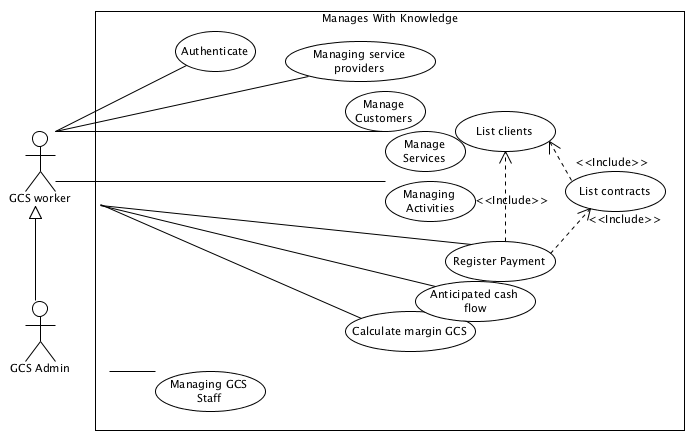
\includegraphics[width=0.9\textwidth]{images/usecase.png}
\caption{The general Usecase of the modelation}\label{img:usecase}
\end{center}
\end{figure} 

\begin{figure}[H]
\begin{center}
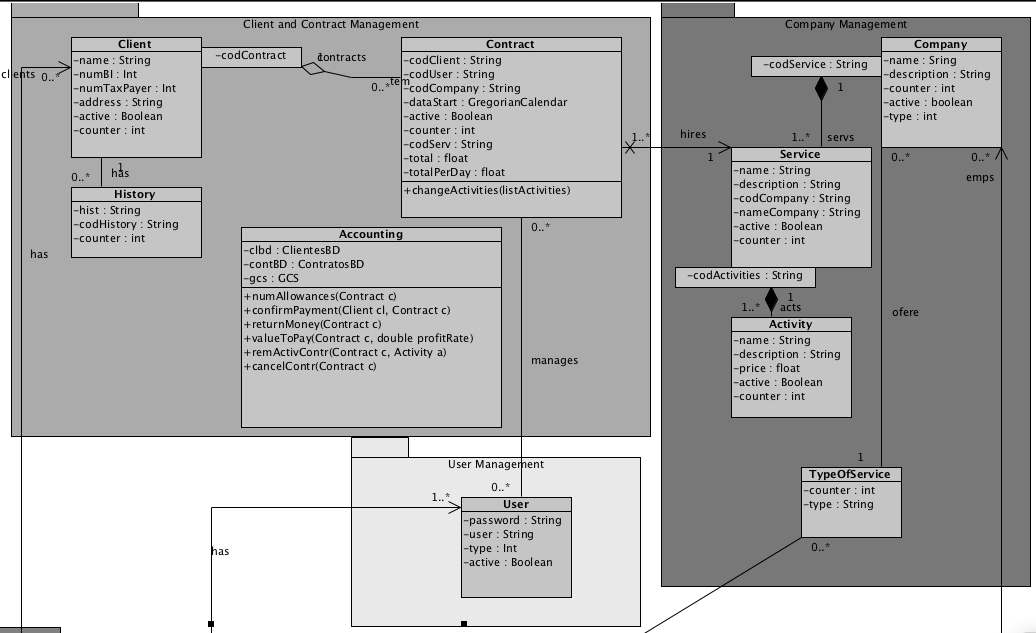
\includegraphics[scale=0.35]{images/classbw.png}
\caption{Excerpt of the Class diagram}\label{img:class}
\end{center}
\end{figure} 
